\begin{document}
\chapter{Overview}
\section{Progressing}
Lorem ipsum dolor sit amet, consectetur adipiscing elit, sed do 
eiusmod tempor incididunt ut labore et dolore magna aliqua. Ut 
enim ad minim veniam, quis nostrud exercitation ullamco...

\subsection{Assignment 1}
Lorem ipsum dolor sit amet, consectetur adipiscing elit, sed do 
eiusmod tempor incididunt ut labore et dolore magna aliqua. Ut 
enim ad minim veniam, quis nostrud exercitation ullamco laboris..

The mass-energy equivalence is described by the famous equation
 
$$E=mc^2$$
 
discovered in 1905 by Albert Einstein. 
In natural units ($c$ = 1), the formula expresses the identity

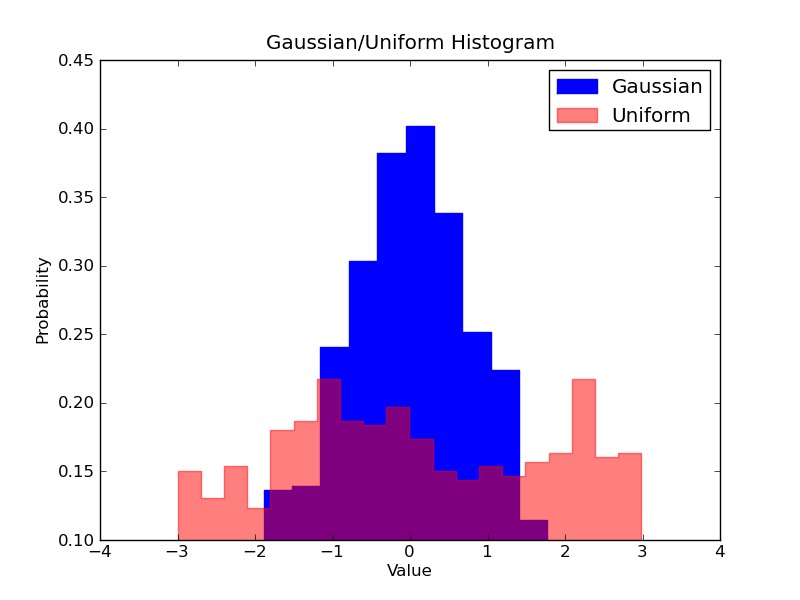
\includegraphics[width=\textwidth]{histogram.png}

\subsection{Assignment 2}
Lorem ipsum dolor sit amet, consectetur adipiscing elit, sed do 
eiusmod tempor incididunt ut labore et dolore magna aliqua. Ut 
enim ad minim veniam, quis nostrud exercitation ullamco laboris..

\section{Obstacles}
Lorem ipsum dolor sit amet, consectetur adipiscing elit, sed do 
eiusmod tempor incididunt ut labore et dolore magna aliqua. Ut 
enim ad minim veniam, quis nostrud exercitation ullamco...

\subsection{Problem 1}
Lorem ipsum dolor sit amet, consectetur adipiscing elit, sed do 
eiusmod tempor incididunt ut labore et dolore magna aliqua. Ut 
enim ad minim veniam, quis nostrud exercitation ullamco laboris..
\begin{itemize}
  \item One entry in the list
  \item Another entry in the list
\end{itemize}
\subsection{Problem 2}
Lorem ipsum dolor sit amet, consectetur adipiscing elit, sed do 
eiusmod tempor incididunt ut labore et dolore magna aliqua. Ut 
enim ad minim veniam, quis nostrud exercitation ullamco laboris..

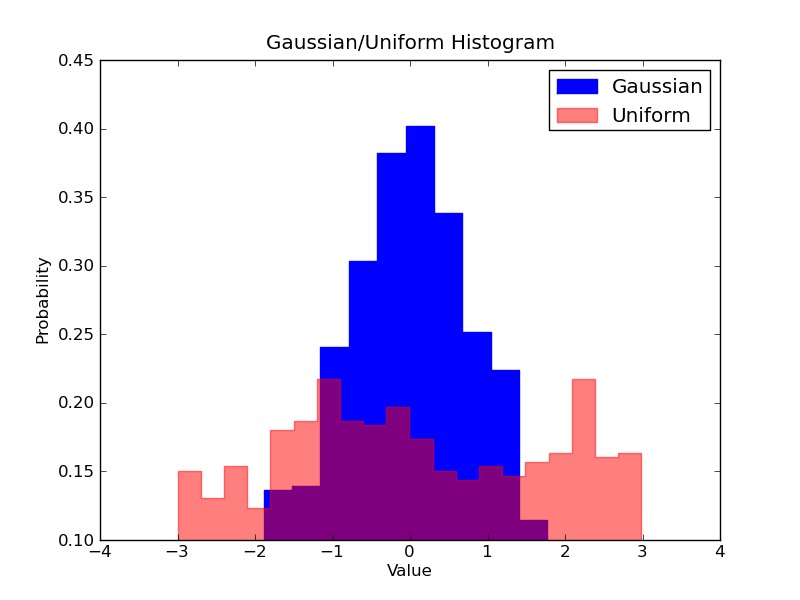
\includegraphics[width=\textwidth]{histogram.png}
\end{document}
